\documentclass[11pt, letterpaper, oneside]{memoir}

\usepackage[T1]{fontenc}
% For typesetting math to mach the Palatino font.
\usepackage{mathpazo}

% For lists.
\usepackage{enumitem}

% For math, such as \aligned.
\usepackage{amsmath}

% To sometimes be able to avoid over full h-boxes.
\usepackage{microtype}

% Graph creation
\usepackage{pgfplots}
%\pgfplotsset{width = 10cm, compat = 1.9}

% For header and footer.
\makepagestyle{plain}
\makeevenfoot{plain}{}{\footnotesize Based on the book Calculus Volume 1. Download for free at https://openstax.org/details/books/calculus-volume-1.}{}
\makeoddfoot{plain}{}{\footnotesize Based on the book Calculus Volume 1. Download for free at https://openstax.org/details/books/calculus-volume-1.}{}

\pagestyle{plain}

\setlrmarginsandblock{3.5cm}{3.5cm}{*}
\setulmarginsandblock{3.5cm}{3.5cm}{*}
\setheadfoot{24pt}{48pt}
\checkandfixthelayout

\begin{document}

\chapter{Functions and Graphs}

\section*{Checkpoint Solutions}

\subsection*{Checkpoint 1.1: Evaluating Functions}

\subsubsection*{Instruction}

For the function $ f(x) = x^2 - 3x + 5 $ evaluate

\begin{enumerate}[label=(\alph*)]
  \item $ f(1) $
  \item $ f(a + h) $
\end{enumerate}

\subsubsection*{Solution}

\begin{enumerate}[label=(\alph*)]
  \item $ f(1) = 1 ^ 2 - 3 \cdot 1 + 5 = 1 - 3 + 5 = 3 $.
  \item $ f(a + h) = (a + h)^2 - 3(a + h) + 5 = a^2 + 2ah + h^2 - 3a - 3h + 5 $.
\end{enumerate}

\subsubsection*{Answer}

\begin{enumerate}[label=(\alph*)]
  \item $ f(1) = 3 $.
  \item $ f(a + h) = a^2 + 2ah + h^2 - 3a - 3h + 5 $.
\end{enumerate}

\subsection*{Checkpoint 1.2: Finding Domain and Range}

\subsubsection*{Instruction}

Find the domain and range for $ f(x) = \sqrt{4 - 2x} + 5 $.

\subsubsection*{Solution}

\begin{enumerate}[label=\roman*]
  \item To find the domain of $ f $, we need the expression $ 4 - 2x \ge 0 $, due to that real negative numbers do not have a square root. Solving this inequality, we conclude that the domain is $ \{ x \mid x \le 2 \} $.
  \item To find the range of $ f $, we note that since $ \sqrt{4 - 2x} \ge 0 $, it follows that $ f(x) = \sqrt{4 - 2x} + 5 \ge 5 $. Therefore, the range of $ f $ must be a subset of the set $ \{ y \mid y \ge 5 \} $.

    To show that every element in this set is in the range of $ f $, we need to show that for all $ y $ in this set, there exists a real number $ x $ in the domain such that $ f(x) = y $. Let $ y \ge 5 $. Then, $ f(x) = y $ if and only if
    $$ \phantom{.}
    \sqrt{4 - 2x} + 5 = y
    .$$
    Solving this equation for $ x $, we see that $ x $ must solve the equation
    $$ \phantom{.}
    \sqrt{4 - 2x}= y - 5
    .$$
    Since $ y \ge 5 $, such an $ x $ could exist. Squaring both sides of the above equation we have
    $$ \phantom{.}
    4-2x = (y - 5)^2
    .$$
    Therefore we need
    $$ \phantom{,}
    -2x= (y - 5)^2 - 4
    ,$$
    which implies
    $$ \phantom{,}
    x= 2 -\frac{(y - 5)^2}{2}
    .$$
    We just need to verify that $ x $ is in the domain of $ f $. Since the domain of $ f $ consists of all real numbers less or equal to $ 2 $, and
    $$ \phantom{,}
    2 -\frac{(y - 5)^2}{2} \le 2
    ,$$
    there does exist an $ x $ in the domain of $ f $. We conclude that the range of $ f $ is $ \{ y \mid y \ge 5 \} $.
\end{enumerate}

\subsubsection*{Answer}

Domain $ = \{ x \mid x \le 2 \} $, range $ = \{ y \mid y \ge 5 \} $.

\subsection*{Checkpoint 1.3: Finding Zeroes}

\subsubsection*{Instruction}

Find the zeroes of $ f(x) = x^3 - 5x^2 + 6x $.

\subsubsection*{Solution}

The zeroes of a function are the values of $ x $ where $ f(x) = 0 $. To find the zeroes, we need to solve
$$ \phantom{.}
f(x) = x^3 - 5x^2 + 6x = 0
.$$
Factor out $ x $
$$ \phantom{.}
f(x) = x(x^2 - 5x + 6) = 0
.$$
We can continue factoring by pure inspection, with the goal of finding a pair of numbers that add up to $ -5 $ and whose product is $ 6 $. This pair of numbers turns out to be $ -2 $ and $ -3 $, leading to the factoring
$$ \phantom{.}
f(x) = x(x - 2)(x - 3) = 0
.$$
From the above complete factoring of $ f $, we conclude that there are three zeroes when $ x $ is 0, 2, and 3.

\subsubsection{Answer}

$ x = 0, 2, 3 $.

\subsection*{Checkpoint 1.4: Combining Functions Using Mathematical Operations}

\subsubsection{Instruction}

For $ f(x) = x^2 + 3 $ and $ g(x) = 2x - 5 $, find $ (f/g)(x) $ and state its domain.

\subsubsection{Solution}

To find $ (f/g)(x) $ we write the function with the quotient operator
$$ \phantom{.}
\frac{f}{g}(x) = \frac{x^2 + 3}{2x - 5}.
$$
The domain of this function is $ \{ x \mid x \ne \frac{5}{2} \} $.

\subsubsection{Answer}

$ \frac{f}{g}(x) = \frac{x^2 + 3}{2x - 5} $. The domain is $ \{ x \mid x \ne \frac{5}{2} \} $.

\subsection*{Checkpoint 1.5: Compositions of Functions}

\subsubsection{Instruction}

Let $ f(x) = 2 - 5x $. Let $ g(x) = \sqrt{x} $. Find $ (f \circ g)(x) $.

\subsubsection{Solution}

$ (f \circ g)(x) = f(g(x)) = f(\sqrt{x}) = 2 - 5\sqrt{x} $.

\subsubsection{Answer}

$ (f \circ g)(x) = 2 - 5\sqrt{x} $.

\subsection*{Checkpoint 1.6: Application Involving a Composite Function}

\subsubsection{Instruction}

If items are on sale for 10\% off their original price, and a customer has a coupon for an additional 30\% off, what will be the final price for an item that is originally x dollars, after applying the coupon to the sale price?

\subsubsection{Solution}

Since the sale price 10\% off the original price, if an item is $ x $ dollars, its sale price is given by
$$ \phantom{.}
f(x) = 0.90x
.$$
Since the coupon entitles an individual to 30\% off the price of any item, if an item is $ y $ dollars, the price after applying the coupon, is given by
$$ \phantom{.}
g(y) = 0.70y
.$$
Therefore, if the price is originally $ x $ dollars, its price after applying the coupon to the sale price will be
$$ \phantom{.}
(g \circ f)(x) = g(f(x)) = (0.70)0.90x = 0.63x.
.$$

\subsubsection{Answer}

$ (g \circ f)(x) = 0.63x $.

\section*{Exercise Solutions}

\subsection*{Exercise 1.1.1}

\subsubsection{Instruction}

Assuming the relation in table \ref{table:exercise-1.1.1}.
\begin{enumerate}[label=(\alph*)]
  \item Determine the domain and the range of the relation.
  \item State whether the relation is a function.
\end{enumerate}

\begin{table}[ht]
  \centering
  \begin{tabular}{ c | r r r r r r r }
    \hline
    $ x $ & $ -3 $ & $ -2 $ & $ -1 $ & $ 0 $ & $ 1 $ & $ 2 $ & $ 3 $ \\
    \hline
    $ y $ & $ 9 $ & $ 4 $ & $ 1 $ & $ 0 $ & $ 1 $ & $ 4 $ & $ 9 $ \\
    \hline
  \end{tabular}
  \caption{Relation between $ x $ and $ y $ in exercise 1.1.1}
  \label{table:exercise-1.1.1}
\end{table}

\subsubsection{Solution}

\begin{enumerate}[label=(\alph*)]
  \item The domain of the relation is the set of unique $ x $ values,
    $$ \phantom{.}
    \{ -3, -2, -1, 0, 1, 2, 3 \}
    .$$
    The range of the relation is the set of unique $ y $ values,
    $$ \phantom{.}
    \{ 0, 1, 4, 9 \}
    .$$
  \item This relation is a function, each input is a assigned to exactly one output.
\end{enumerate}

\subsubsection{Answer}

\begin{enumerate}[label=(\alph*)]
  \item Domain = $ \{ -3, -2, -1, 0, 1, 2, 3 \} $, range = $ \{ 0, 1, 4, 9 \} $.
  \item Yes, a function.
\end{enumerate}

\subsection*{Exercise 1.1.2}

\subsubsection{Instruction}

Assuming the relation in table \ref{table:exercise-1.1.2}.
\begin{enumerate}[label=(\alph*)]
  \item Determine the domain and the range of the relation.
  \item State whether the relation is a function.
\end{enumerate}

\begin{table}[ht]
  \centering
  \begin{tabular}{ c | r r r r r r r }
    \hline
    $ x $ & $ -3 $ & $ -2 $ & $ -1 $ & $ 0 $ & $ 1 $ & $ 2 $ & $ 3 $ \\
    \hline
    $ y $ & $ -2 $ & $ -8 $ & $ -1 $ & $ 0 $ & $ 1 $ & $ 8 $ & $ -2 $ \\
    \hline
  \end{tabular}
  \caption{Relation between $ x $ and $ y $ in exercise 1.1.2}
  \label{table:exercise-1.1.2}
\end{table}

\subsubsection{Solution}

\begin{enumerate}[label=(\alph*)]
  \item The domain of the relation is the set of unique $ x $ values,
    $$ \phantom{.}
    \{ -3, -2, -1, 0, 1, 2, 3 \}
    .$$
    The range of the relation is the set of unique $ y $ values,
    $$ \phantom{.}
    \{ -8, -2, -1, 0, 1, 8\}
    .$$
  \item This relation is a function, each input is a assigned to exactly one output.
\end{enumerate}

\subsubsection{Answer}

\begin{enumerate}[label=(\alph*)]
  \item Domain = $ \{ -3, -2, -1, 0, 1, 2, 3 \} $, range = $ \{ -8, -2, -1, 0, 1, 8\} $.
  \item Yes, a function.
\end{enumerate}

\subsection*{Exercise 1.1.3}

\subsubsection{Instruction}

Assuming the relation in table \ref{table:exercise-1.1.3}.
\begin{enumerate}[label=(\alph*)]
  \item Determine the domain and the range of the relation.
  \item State whether the relation is a function.
\end{enumerate}

\begin{table}[ht]
  \centering
  \begin{tabular}{ c | r r r r r r r }
    \hline
    $ x $ & $ 1 $ & $ 2 $ & $ 3 $ & $ 0 $ & $ 1 $ & $ 2 $ & $ 3 $ \\
    \hline
    $ y $ & $ -3 $ & $ -2 $ & $ -1 $ & $ 0 $ & $ 1 $ & $ 2 $ & $ 3 $ \\
    \hline
  \end{tabular}
  \caption{Relation between $ x $ and $ y $ in exercise 1.1.3}
  \label{table:exercise-1.1.3}
\end{table}

\subsubsection{Solution}

\begin{enumerate}[label=(\alph*)]
  \item The domain of the relation is the set of unique $ x $ values,
    $$ \phantom{.}
    \{ 0, 1, 2, 3 \}
    .$$
    The range of the relation is the set of unique $ y $ values,
    $$ \phantom{.}
    \{ -3, -2, -1, 0, 1, 2, 3 \}
    .$$
  \item This relation is not a function, each input is not assigned to exactly one output. Take for example $ x = 1 $ that can cause both $ y = -3 $ and $ y = 1 $.
\end{enumerate}

\subsubsection{Answer}

\begin{enumerate}[label=(\alph*)]
  \item Domain = $ \{ 0, 1, 2, 3 \} $, range = $ \{ -3, -2, -1, 0, 1, 2, 3 \} $.
  \item No, not a function.
\end{enumerate}

\subsection*{Exercise 1.1.4}

\subsubsection{Instruction}

Assuming the relation in table \ref{table:exercise-1.1.4}.
\begin{enumerate}[label=(\alph*)]
  \item Determine the domain and the range of the relation.
  \item State whether the relation is a function.
\end{enumerate}

\begin{table}[ht]
  \centering
  \begin{tabular}{ c | r r r r r r r }
    \hline
    $ x $ & $ 1 $ & $ 2 $ & $ 3 $ & $ 4 $ & $ 5 $ & $ 6 $ & $ 7 $ \\
    \hline
    $ y $ & $ 1 $ & $ 1 $ & $ 1 $ & $ 1 $ & $ 1 $ & $ 1 $ & $ 1 $ \\
    \hline
  \end{tabular}
  \caption{Relation between $ x $ and $ y $ in exercise 1.1.4}
  \label{table:exercise-1.1.4}
\end{table}

\subsubsection{Solution}

\begin{enumerate}[label=(\alph*)]
  \item The domain of the relation is the set of unique $ x $ values,
    $$ \phantom{.}
    \{ 1, 2, 3, 4, 5, 6, 7 \}
    .$$
    The range of the relation is the set of unique $ y $ values,
    $$ \phantom{.}
    \{ 1 \}
    .$$
  \item This relation is a function, each input is a assigned to exactly one output.
\end{enumerate}

\subsubsection{Answer}

\begin{enumerate}[label=(\alph*)]
  \item Domain = $  \{ 1, 2, 3, 4, 5, 6, 7 \} $, range = $ \{ 1 \} $.
  \item Yes, a function.
\end{enumerate}

\subsection*{Exercise 1.1.5}

\subsubsection{Instruction}

Assuming the relation in table \ref{table:exercise-1.1.5}.
\begin{enumerate}[label=(\alph*)]
  \item Determine the domain and the range of the relation.
  \item State whether the relation is a function.
\end{enumerate}

\begin{table}[ht]
  \centering
  \begin{tabular}{ c | r r r r r r r }
    \hline
    $ x $ & $ 3 $ & $ 5 $ & $ 8 $ & $ 10 $ & $ 15 $ & $ 21 $ & $ 33 $ \\
    \hline
    $ y $ & $ 3 $ & $ 2 $ & $ 1 $ & $ 0 $ & $ 1 $ & $ 2 $ & $ 3 $ \\
    \hline
  \end{tabular}
  \caption{Relation between $ x $ and $ y $ in exercise 1.1.5}
  \label{table:exercise-1.1.5}
\end{table}

\subsubsection{Solution}

\begin{enumerate}[label=(\alph*)]
  \item The domain of the relation is the set of unique $ x $ values,
    $$ \phantom{.}
    \{ 3, 5, 8, 10, 15, 21, 33 \}
    .$$
    The range of the relation is the set of unique $ y $ values,
    $$ \phantom{.}
    \{ 0, 1, 2, 3\}
    .$$
  \item This relation is a function, each input is a assigned to exactly one output.
\end{enumerate}

\subsubsection{Answer}

\begin{enumerate}[label=(\alph*)]
  \item Domain = $  \{ 3, 5, 8, 10, 15, 21, 33 \} $, range = $ \{ 0, 1, 2, 3\} $.
  \item Yes, a function.
\end{enumerate}

\subsection*{Exercise 1.1.6}

\subsubsection{Instruction}

Assuming the relation in table \ref{table:exercise-1.1.6}.
\begin{enumerate}[label=(\alph*)]
  \item Determine the domain and the range of the relation.
  \item State whether the relation is a function.
\end{enumerate}

\begin{table}[ht]
  \centering
  \begin{tabular}{ c | r r r r r r r }
    \hline
    $ x $ & $ -7 $ & $ -2 $ & $ -2 $ & $ 0 $ & $ 1 $ & $ 3 $ & $ 6 $ \\
    \hline
    $ y $ & $ 11 $ & $ 5 $ & $ 1 $ & $ -1 $ & $ -2 $ & $ 4 $ & $ 11 $ \\
    \hline
  \end{tabular}
  \caption{Relation between $ x $ and $ y $ in exercise 1.1.6}
  \label{table:exercise-1.1.6}
\end{table}

\subsubsection{Solution}

\begin{enumerate}[label=(\alph*)]
  \item The domain of the relation is the set of unique $ x $ values,
    $$ \phantom{.}
    \{ -7, -2, 0, 1, 3, 6 \}
    .$$
    The range of the relation is the set of unique $ y $ values,
    $$ \phantom{.}
    \{ -2, -1, 1, 4, 5, 11\}
    .$$
  \item This relation is not a function, each input is not assigned to exactly one output. See $ x = -2, $ that can cause both $ y = 1 $ and $ y = 5 $.
\end{enumerate}

\subsubsection{Answer}

\begin{enumerate}[label=(\alph*)]
  \item Domain = $  \{ -7, -2, 0, 1, 3, 6 \} $, range = $ \{ -2, -1, 1, 4, 5, 11\} $.
  \item No, not a function.
\end{enumerate}

\subsection*{Exercise 1.1.7}

\subsubsection{Instruction}

Find the below values for the function $ f(x) = 5x - 2 $, if they exist, then simplify.
\begin{enumerate}[label=(\alph*)]
  \item $ f(0) $
  \item $ f(1) $
  \item $ f(3) $
  \item $ f(-x) $
  \item $ f(a) $
  \item $ f(a + h) $
\end{enumerate}

\subsubsection{Solution}

\begin{enumerate}[label=(\alph*)]
  \item $ f(0) = 5 \cdot 0 - 2 = 0 - 2 = -2 $.
  \item $ f(1) = 5 \cdot 1 - 2 = 5 - 2 = 3 $.
  \item $ f(2) = 5 \cdot 3 - 2 = 15 - 2 = 13 $.
  \item $ f(-x) = 5(-x) - 2 = -5x - 2 $.
  \item $ f(a) = 5a - 2 $.
  \item $ f(a + h) = 5(a + h) - 2 = 5a + 5h - 2 $.
\end{enumerate}

\subsubsection{Answer}

\begin{enumerate}[label=(\alph*)]
  \item $ -2 $.
  \item $ 3 $.
  \item $ 13 $.
  \item $ -5x - 2 $.
  \item $ 5a - 2 $.
  \item $ 5a + 5h - 2$.
\end{enumerate}

\subsection*{Exercise 1.1.8}

\subsubsection{Instruction}

Find the below values for the function $ f(x) = 4x^2 - 3x + 1 $, if they exist, then simplify.
\begin{enumerate}[label=(\alph*)]
  \item $ f(0) $
  \item $ f(1) $
  \item $ f(3) $
  \item $ f(-x) $
  \item $ f(a) $
  \item $ f(a + h) $
\end{enumerate}

\subsubsection{Solution}

\begin{enumerate}[label=(\alph*)]
  \item $ f(0) = 4 \cdot 0^2 - 3 \cdot 0 + 1 = 4 \cdot 0 - 0 + 1 = 0 - 0 + 1 = 1 $.
  \item $ f(1) = 4 \cdot 1^2 - 3 \cdot 1 + 1 = 4 \cdot 1 - 3 + 1 = 4 - 3 + 1 = 2 $.
  \item $ f(3) = 4 \cdot 3^2 - 3 \cdot 3 + 1 = 4 \cdot 9 - 9 + 1 = 36 - 9 + 1 = 28 $.
  \item $ f(-x) = 4(-x)^2 - 3(-x) + 1 = 4x^2 + 3x + 1 $.
  \item $ f(a) = 4a^2 - 3a + 1 $.
  \item
    \(
      \begin{aligned}[t]
        f(a + h) &= 4(a + h)^2 - 3(a + h) + 1 \\
        &= 4(a^2 + 2ah + h^2) - 3a - 3h + 1 \\
        &= 4a^2 + 4h^2 + 8ah -3a - 3h + 1.
      \end{aligned}
    \)

\end{enumerate}

\subsubsection{Answer}

\begin{enumerate}[label=(\alph*)]
  \item $ 1 $.
  \item $ 2 $.
  \item $ 28 $.
  \item $ 4x^2 + 3x + 1 $.
  \item $ 4a^2 - 3a + 1 $.
  \item $ 4a^2 + 4h^2 + 8ah -3a - 3h + 1 $.
\end{enumerate}

\subsection*{Exercise 1.1.15}

Find the domain, range, and all zeros/intercepts, if any, of the function $ g(x) = \sqrt{8x - 1} $.

\subsubsection{Solution}

\begin{enumerate}[label=\roman*]

  \item
    The domain of the square root function is $ \left[ 0, \infty \right) $, which implies $ 8x - 1 \ge 0 $. Solving for $ x $ gives $ x \ge \frac{1}{8} $.

  \item
    To find the range of $ g $, we note that $ \sqrt{8x - 1} \ge 0 $. Therefore, the range of $ g $ must be a subset of the set $ \{y \mid y \ge 0\} $. To show that every element in this set is in the range of $ g $, we need to show that for a given $ y $ in this set, there exists a real number $ x $ in the domain such that $ g(x) = y $.

    Let $ y \ge 0 $. Then $ g(x) = y $ if and only if
    $$ \phantom{.}
    \sqrt{8x - 1} = y
    .$$

    We are interested in $ x $, and will solve this equation for $ x $. Since $ y \ge 0 $ such an $ x $ could exist. Squaring both sides of this equation, we have
    $$ \phantom{.}
    {8x - 1} = y^2
    .$$
    Therefore, we need
    $$ \phantom{.}
    8x = y^2 + 1
    ,$$
    which implies
    $$ \phantom{.}
    x = \frac{y^2 + 1}{8}
    .$$
    We just need to verify that $ x $ is in the domain of $ g $. Since the domain of $ g $ consists of all real numbers greater than or equal to $ 1 / 8 $, and
    $$ \phantom{.}
    \frac{y^2 + 1}{8} \ge \frac{1}{8}
    ,$$
    there does exist an $ x $ in the domain of $ g $. We conclude that the range of $ g $ is $ \{ y \mid y \ge 0 \} $.

  \item
    To find the zeroes, solve $ g(x) = \sqrt{8x - 1}0 $. We discover that $ g $ have one zero at $ x = -1/8 $.

  \item The y-intercept is given by $ (0, g(0)) $. Since $ x = 0 $ isn't in the domain of $ g $, it follows that that there aren't any intercepts.

\end{enumerate}

\subsubsection{Answer}

Domain = $ x \ge \frac{1}{8} $, range = $ \{ y \mid y \ge 0 \} $, zeroes $ x = -1/8 $, no intercepts.

\subsection*{Exercise 1.1.23}

Sketch the graph for the function $ f(x) = 3x - 6 $ with the aid of table \ref{table:exercise-1.1.23}.

\begin{table}[ht]
  \centering
  \begin{tabular}{ c | r r r r r r r }
    \hline
    $ x $ & $ -3 $ & $ -2 $ & $ -1 $ & $ 0 $ & $ 1 $ & $ 2 $ & $ 3 $ \\
    \hline
    $ y $ & $ -15 $ & $ -12 $ & $ -9 $ & $ -6 $ & $ -3 $ & $ 0 $ & $ 3 $ \\
    \hline
  \end{tabular}
  \caption{Relation between $ x $ and $ y $ in exercise 1.1.23}
  \label{table:exercise-1.1.23}
\end{table}

\subsubsection{Solution}

Begin by sketching the axes. We choose the same scale on both axes to not distort the graph. We choose the range for both axes to be -15 to 15, allowing us to plot all the points from table \ref{table:exercise-1.1.23}. See figure \ref{figure:exercise-1.1.23-figure-1}.

\bigskip
\begin{figure}[!h]
  \centering
  \begin{tikzpicture}
    \centering
    \begin{axis}[
        axis x line = center,
        axis y line = center,
        xlabel = \( x \),
        ylabel = \( y \),
        xmin = -17.5, xmax = 17.5,
        ymin = -17.5, ymax = 17.5,
        xtick distance = 5,
        ytick distance = 5,
      ]
    \end{axis}
  \end{tikzpicture}
  \caption{Empty graph with just the axes}
  \label{figure:exercise-1.1.23-figure-1}
\end{figure}
\bigskip

After having sketched the axes we add markers based on the data in table \ref{table:exercise-1.1.23}. See figure \ref{figure:exercise-1.1.23-figure-2}.

\bigskip
\begin{figure}[!h]
  \centering
  \begin{tikzpicture}
    \centering
    \begin{axis}[
        axis x line = center,
        axis y line = center,
        xlabel = \( x \),
        ylabel = \( y \),
        xmin = -17.5, xmax = 17.5,
        ymin = -17.5, ymax = 17.5,
        xtick distance = 5,
        ytick distance = 5,
      ]
      \addplot[
        only marks,
        color = blue,
        mark = *,
      ]
      coordinates {
        (-3,-15)(-2,-12)(-1,-9)(0,-6)(1,-3)(2,0)(3,3)
      };
    \end{axis}
  \end{tikzpicture}
  \caption{Graph with added markers}
  \label{figure:exercise-1.1.23-figure-2}
\end{figure}
\bigskip

We then connect the markers with line segments. In this particular case the result will be a single straight line so we can use a ruler when sketching.

\begin{figure}[!h]
  \centering
  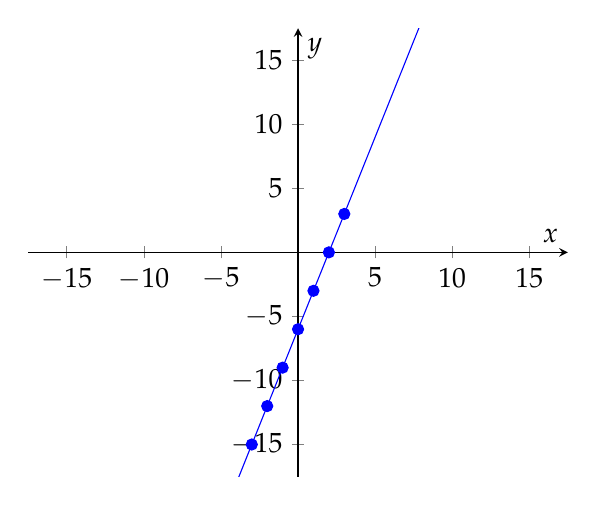
\begin{tikzpicture}
    \centering
    \begin{axis}[
        axis x line = center,
        axis y line = center,
        xlabel = \( x \),
        ylabel = \( y \),
        xmin = -17.5, xmax = 17.5,
        ymin = -17.5, ymax = 17.5,
        xtick distance = 5,
        ytick distance = 5,
      ]
      \addplot[
        only marks,
        color = blue,
        mark = *,
      ]
      coordinates {
        (-3,-15)(-2,-12)(-1,-9)(0,-6)(1,-3)(2,0)(3,3)
      };
      \addplot [
        domain=-17.5:17.5,
        samples=100,
        color=blue,
      ]
      {3 * x - 6};
    \end{axis}
  \end{tikzpicture}
  \caption{Graph with connected markers}
\end{figure}

\subsubsection*{Answer}

\begin{figure}[!h]
  \centering
  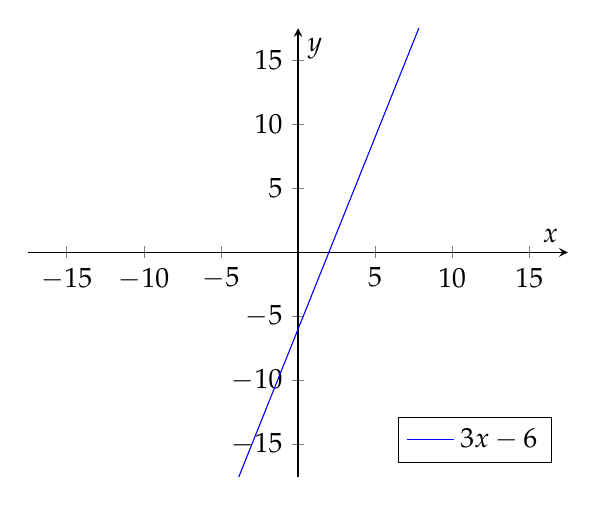
\begin{tikzpicture}
    \centering
    \begin{axis}[
        axis x line = center,
        axis y line = center,
        xlabel = \( x \),
        ylabel = \( y \),
        xmin = -17.5, xmax = 17.5,
        ymin = -17.5, ymax = 17.5,
        xtick distance = 5,
        ytick distance = 5,
        legend pos = south east,
      ]
      \addplot [
        domain=-17.5:17.5,
        samples=100,
        color=blue,
      ]
      {3 * x - 6};
      \addlegendentry{\( 3x - 6 \)}
    \end{axis}
  \end{tikzpicture}
  \caption{Answer to exercise 1.1.23}
\end{figure}

\end{document}
